\section{\label{I-B-2}Conséquences pratiques : l'exemple de la migration vers la plateforme \gls{clade}}

Durant les missions réalisées lors de ce stage, cette contrainte s'est particulièrement manifestée dans l'imposition d'outils informatiques de catalogage et de diffusion des collections au \mae. Les chantiers de mise en place de nouveaux logiciels, achevés durant l'été 2025, ont tous deux été pilotés par le \minarm : l'implémentation du logiciel de gestion des collections \gls{archange} (\textit{S-Museum} de \textit{Skinsoft}) s'inscrit dans un projet progressif d'intégration des musées du ministère sur une même plateforme de gestion des collections. La migration vers le \ac{sigb} \gls{koha} pour la bibliothèque, et la diffusion de ses collections sur la plateforme \gls{clade}, s'inscrit dans un projet similaire visant à unifier la gestion de toutes les bibliothèques du ministère et à améliorer leur accessibilité en permettant à l'utilisateur d'interroger l'ensemble des \gls{bibmusee} sur un portail unique.

Cette situation peut placer le musée dans des positions délicates : dans le cas de la migration vers \gls{clade}, à laquelle j'ai été confrontée durant mon stage, les responsables du \ac{drd} ont dû faire face à des difficultés particulières, directement causées par l'intégration de la bibliothèque du \mae à un réseau plus large. D'une part, ce projet offre des avantages considérables en matière d'accessibilité des catalogues : centralisation de la recherche, recherche par mots-clés, intégration de documents numériques téléchargeables\footcite{ministeredesarmeesKitCommunicationCLADE}. Il permet également à des institutions plus modestes de participer à un projet qu'elles n'auraient peut-être pas eu les ressources de mener indépendamment. D'autre part, cela rend plus délicat l'adaptation aux exigences et aux habitudes de gestion spécifiques à chaque institution, ce qui devient problématique pour des bibliothèques spécialisées comme celle du \mae.

Par exemple, la gestion ministérielle du projet a privé les agents du \ac{drd} de visibilité sur son déroulement : ils n'ont jamais eu accès au cahier des charges du projet. Il devient alors difficile pour les utilisateurs d'identifier d'éventuels problèmes pendant la migration : ce n'est qu'à la fin de la phase de test qu'a été découvert que la structure du fichier d'import du thésaurus avait été mal comprise par les responsables de la migration des données, causant des inexactitudes lors de l'import, extrêmement difficiles à corriger a posteriori.

Au-delà des problèmes d'import, la configuration même d'une telle plateforme représente de réels défis, qui ne sont pas encore pleinement résolus : comme le manifestent les captures d'écran de l'interface web ci-dessous\footnote{Voir la figure \ref{fig:clade_histoaviation}}, \gls{clade} offre une interface moderne et ergonomique. Celle-ci permet d'effectuer des recherches par mot-clé et par institution (appelées \enquote{portails}). Des filtres permettent de préciser la recherche et chaque utilisateur peut se constituer un panier, sauvegarder des favoris\dots autant de fonctionnalités qui n'existaient pas de manière aussi avancées dans l'ancien logiciel \gls{alexandrie}. Un nuage de mots-clés permet même d'avoir un aperçu rapide des connaissances englobées par la recherche de l'utilisateur. En se penchant sur les notices, le défi représenté par ce regroupement -- et les exigences d'interopérabilité qui en découlent pour le \mae -- devient manifeste : chaque institution ayant ses habitudes de catalogage propres, réconcilier les différents ouvrages devient difficile lorsque la mise en forme du contenu des champs, les champs eux-mêmes et la structuration du thésaurus diffèrent d'un même ouvrage à l'autre selon le producteur de la notice.


\begin{figure}[htbp]
	\centering
	\begin{subfigure}{0.7\textwidth}
		\centering
		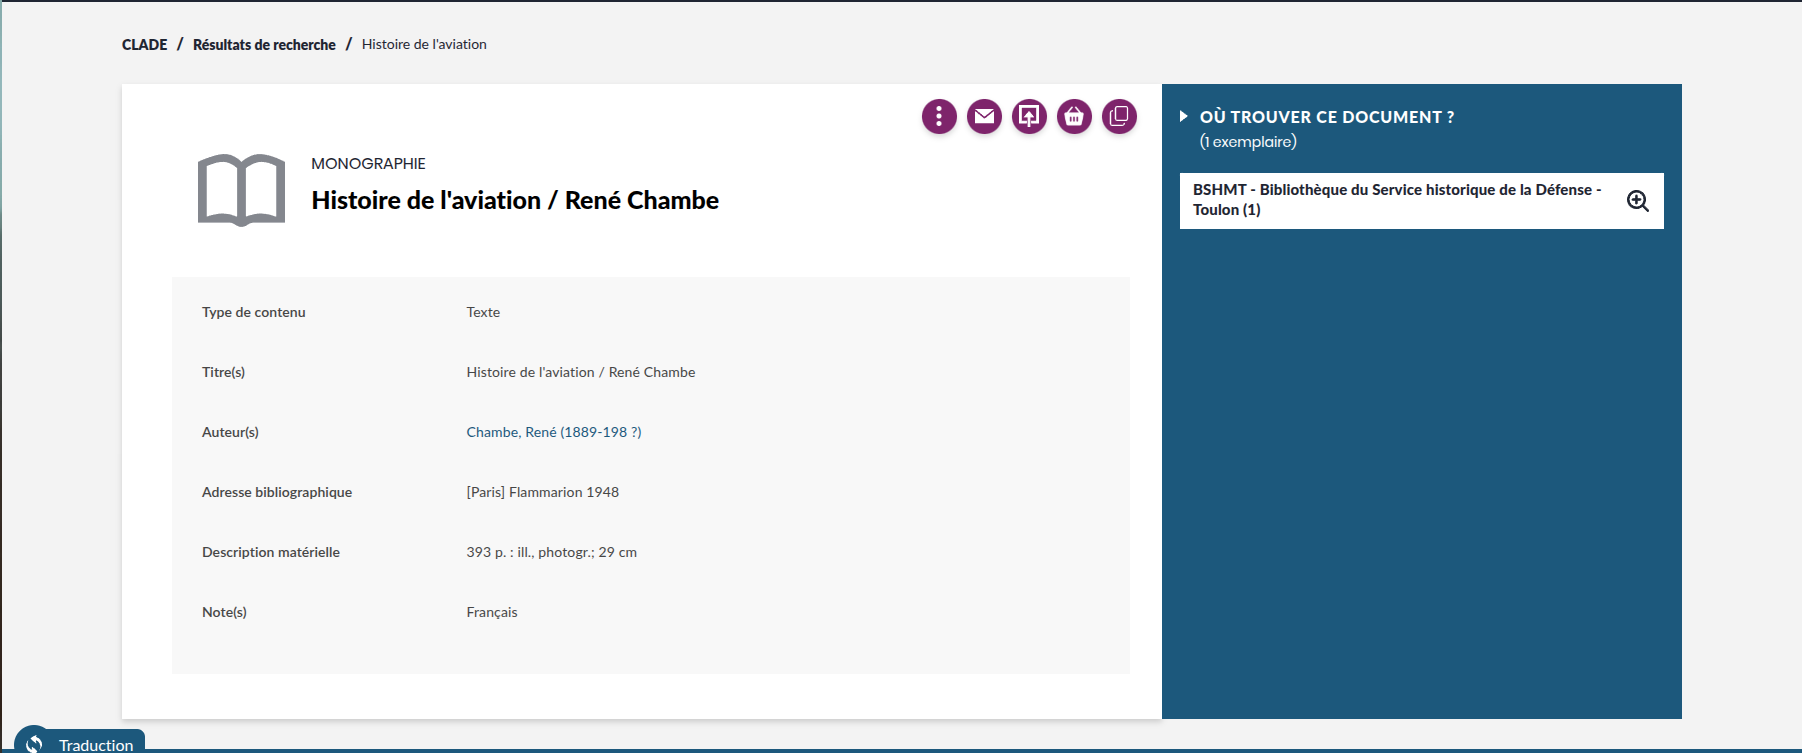
\includegraphics[width=\linewidth]{img/IMG_clade_histoireaviation_shdTL}
		\caption{Service Historique de la Défense}
		\label{img:cladehistoireaviationshdtl}
	\end{subfigure}
	\begin{subfigure}{0.7\textwidth}
		\centering
		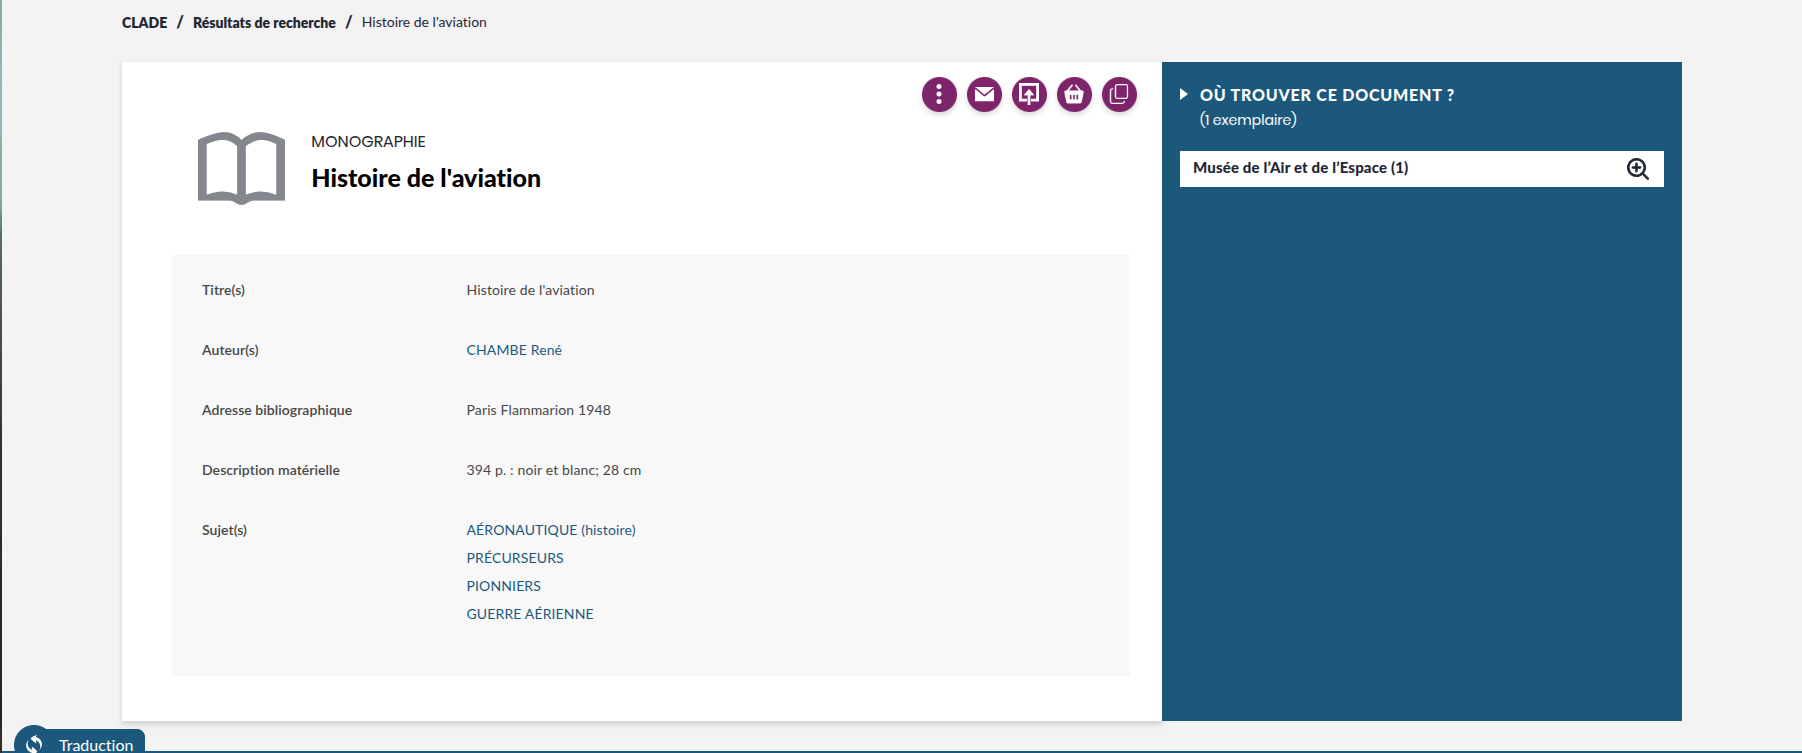
\includegraphics[width=\linewidth]{img/IMG_clade_histoireaviation_mae}
		\caption{\mae}
		\label{img:cladehistoireaviationsmae}
	\end{subfigure}
	\hfill
	\begin{subfigure}{0.7\textwidth}
		\centering
		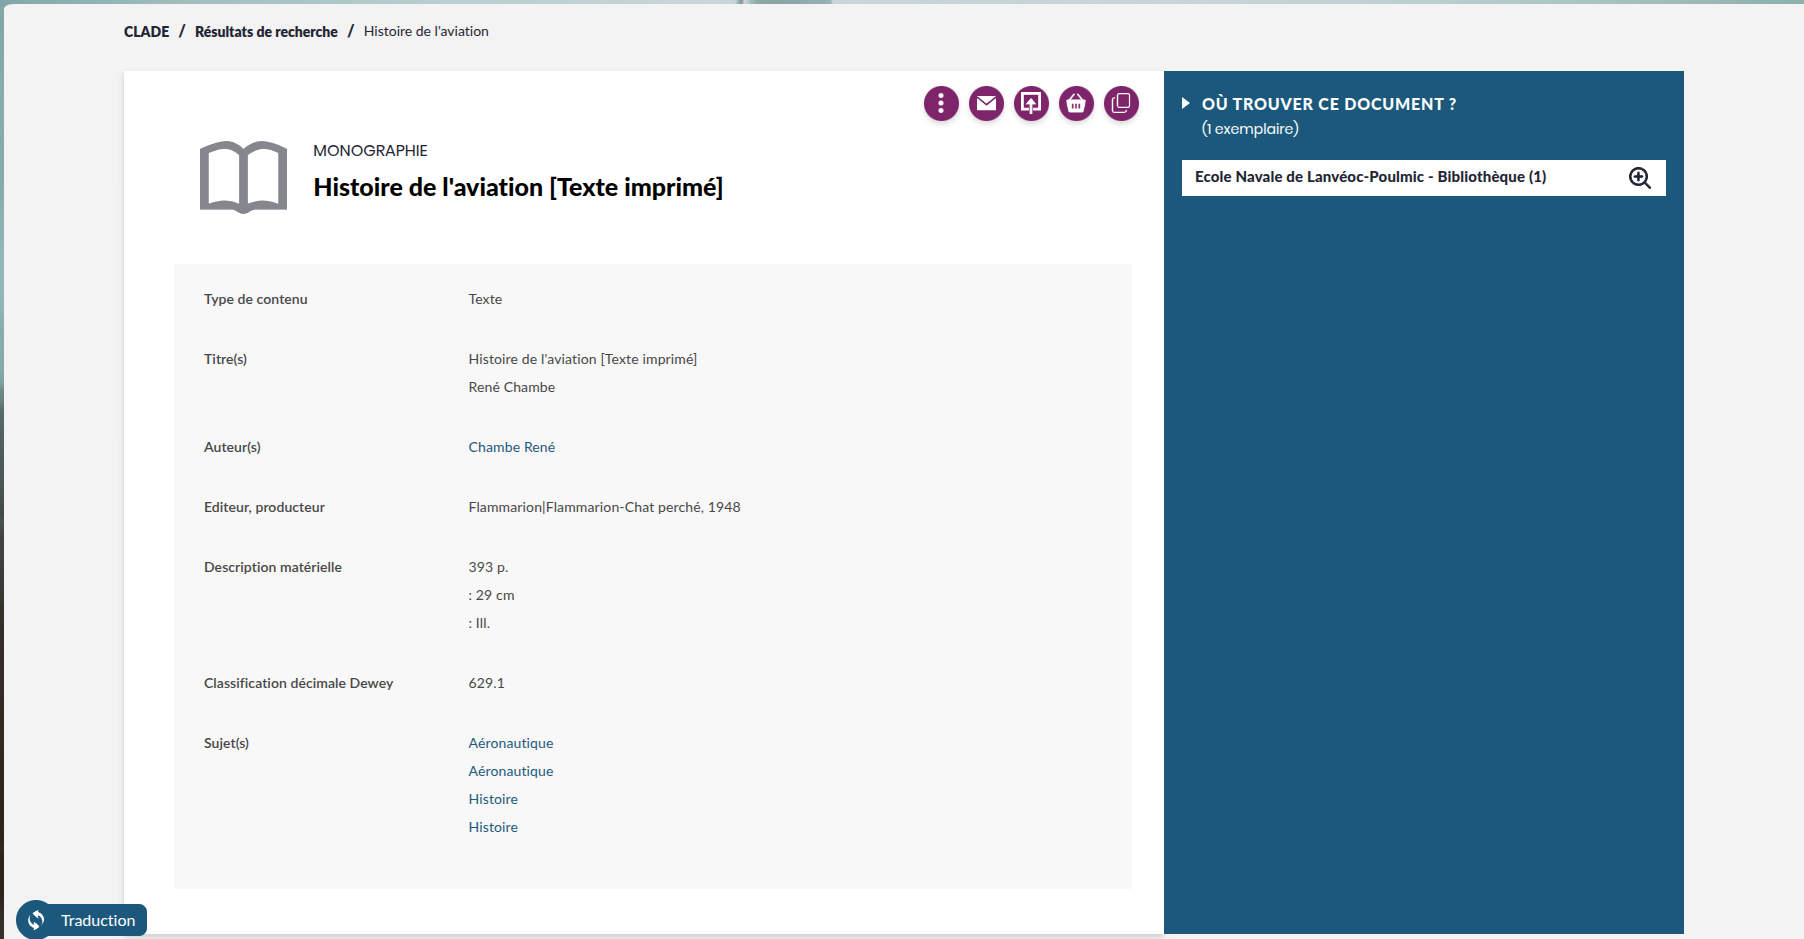
\includegraphics[width=\linewidth]{img/IMG_clade_histoireaviation_navale}
		\caption{École navale}
		\label{img:cladehistoireaviationnavale}
	\end{subfigure}
	\caption[Différences de catalogage entre les \bibmusee sur \ac{clade}]{Malgré la volonté de mise en commun sur \ac{clade}, la même édition d'un même ouvrage peut être cataloguée de plusieurs manières différentes et apparaître comme des ouvrages distincts : ici, l'\textit{Histoire de l'aviation} de René Chambe chez Flammarion (1948)}
	\label{fig:clade_histoaviation}
\end{figure}

Ce cas illustre parfaitement les tensions inhérentes aux vocabulaires contrôlés en contexte institutionnel contraint : l'harmonisation impose des choix qui peuvent entrer en conflit avec les besoins documentaires spécifiques, et pose la question de trouver comment accorder les richesses des connaissances de chaque institution concernée avec la nécessité d'avoir un minimum d'uniformité lorsqu'il s'agit de coopérer à grande échelle. Cette expérience pose des questions que nous développerons dans les parties suivantes : quels critères peuvent guider la conception de vocabulaires contrôlés qui articulent contraintes institutionnelles et exigences scientifiques ? Comment évaluer les compromis entre interopérabilité et précision sémantique ? Comment trouver un équilibre entre intéropérabilité et fidélité à l'identité et à la valeur scientifique des collections ?